\begin{figure}[H]
    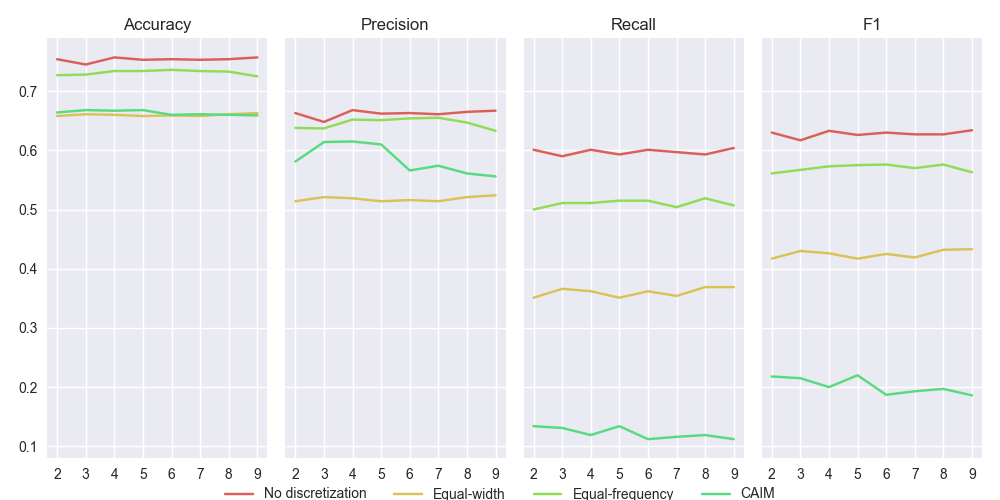
\includegraphics[width=\textwidth]{img/cv_scores_kfold/scoring_kfold_diabetes.png}
    \caption{Wykresy wartości metryk dla zbioru "Diabetes" -- krowalidacja zwykła.}
\end{figure}

 \begin{table}[H]
    \center
    \caption{Wartości metryk dla zbioru "Diabetes" -- krowalidacja zwykła.}
    \begin{tabular}{|c|c|c|c|c|c|c|c|c|c|}
        \hline
        \multirow{2}{*}{\textbf{Metoda dyskr.}} & \multirow{2}{*}{\textbf{Metryka}} & \multicolumn{8}{|c|}{\textbf{CV}} \\ \cline{3-10}
                                                &  & 2 & 3 & 4 & 5 & 6 & 7 & 8 & 9 \\ \hline
            \multirow{4}{*}{\textit{Brak}}  & Accuracy & 0.754 & 0.745 & 0.757 & 0.753 & 0.754 & 0.753 & 0.754 & 0.757 \\ \cline{2-10}
                                             & Precision & 0.663 & 0.648 & 0.668 & 0.662 & 0.663 & 0.661 & 0.665 & 0.667 \\ \cline{2-10}
                                             & Recall & 0.601 & 0.59 & 0.601 & 0.593 & 0.601 & 0.597 & 0.593 & 0.604 \\ \cline{2-10}
                                             & F1 & 0.63 & 0.617 & 0.633 & 0.626 & 0.63 & 0.627 & 0.627 & 0.634 \\ \hline  \hline


                                            \multirow{4}{*}{\textit{Equal-width}}  & Accuracy & 0.658 & 0.661 & 0.66 & 0.658 & 0.659 & 0.658 & 0.661 & 0.663 \\ \cline{2-10}
                                             & Precision & 0.514 & 0.521 & 0.519 & 0.514 & 0.516 & 0.514 & 0.521 & 0.524 \\ \cline{2-10}
                                             & Recall & 0.351 & 0.366 & 0.362 & 0.351 & 0.362 & 0.354 & 0.369 & 0.369 \\ \cline{2-10}
                                             & F1 & 0.417 & 0.43 & 0.426 & 0.417 & 0.425 & 0.419 & 0.432 & 0.433 \\ \hline  \hline


                                            \multirow{4}{*}{\textit{Equal-freq}}  & Accuracy & 0.727 & 0.728 & 0.734 & 0.734 & 0.736 & 0.734 & 0.733 & 0.725 \\ \cline{2-10}
                                             & Precision & 0.638 & 0.637 & 0.652 & 0.651 & 0.654 & 0.655 & 0.647 & 0.633 \\ \cline{2-10}
                                             & Recall & 0.5 & 0.511 & 0.511 & 0.515 & 0.515 & 0.504 & 0.519 & 0.507 \\ \cline{2-10}
                                             & F1 & 0.561 & 0.567 & 0.573 & 0.575 & 0.576 & 0.57 & 0.576 & 0.563 \\ \hline  \hline


                                            \multirow{4}{*}{\textit{CAIM}}  & Accuracy & 0.664 & 0.668 & 0.667 & 0.668 & 0.66 & 0.661 & 0.66 & 0.659 \\ \cline{2-10}
                                             & Precision & 0.581 & 0.614 & 0.615 & 0.61 & 0.566 & 0.574 & 0.561 & 0.556 \\ \cline{2-10}
                                             & Recall & 0.134 & 0.131 & 0.119 & 0.134 & 0.112 & 0.116 & 0.119 & 0.112 \\ \cline{2-10}
                                             & F1 & 0.218 & 0.215 & 0.2 & 0.22 & 0.187 & 0.193 & 0.197 & 0.186 \\ \hline  \hline
            \hline
        \end{tabular}
    \end{table}

\begin{figure}[H]
    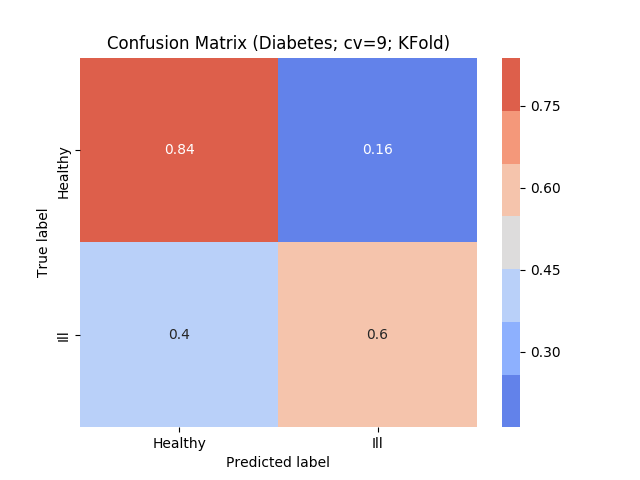
\includegraphics[width=\textwidth]{img/conf_matrices/cm_Diabetes_cv9_KFold.png}
    \caption{Macierz konfuzji dla najlepszej wartości F1 -- kroswalidacja zwykła.}
\end{figure}